\section{Evaluating the surrogate library and ensemble}
\label{sec:experiments}
\subsection{Datasets and comparison coverage}
We assemble a benchmark of 22 datasets spanning elliptic equations, diffusion,
convection, shocks, porous flow, reaction diffusion, waves, and ERA5 climate
emulation \citep{hersbach2020,niu2024}. Figure~\ref{fig:datasets} shows one fine
field from each dataset, illustrating the range of field structures and grid
resolutions. The collection combines our simulations with
imported parameter and field data, using different grids or data sources as
fidelities. Euler, Burgers, and Shallow water use the published PyClaw finite
volume framework \citep{ketcheson2012pyclaw}. Their problem designs include
Euler quadrant configurations motivated by The Well \citep{ohana2024} and a
radial dam break adapted from PDEBench \citep{takamoto2022}. Custom solvers
are supported by targeted analytical and numerical checks, including a
Barenblatt solution test for Porous medium and mesh refinement for Allen Cahn
(Appendix~\ref{app:generatorchecks}). Several datasets describe the same governing equation, so the
roster represents 22 prediction tasks rather than 22 independent physical
families (Appendix~\ref{app:roster}).

We evaluate all nine library models and their ensembles on all 22 datasets.
Models are trained using the training examples available for each dataset,
with additional fine examples reserved for ensemble fitting. Reported
comparisons use the same evaluation cases within each dataset and fitting
partition. Each final surrogate model uses a single seed. Baseline settings, model
specific training schedules, fitting and validation allocations, and comparison
coverage are detailed in Appendices~\ref{app:protocol}
and~\ref{app:matchedbaselines}.

\begin{figure}[t]
\centering
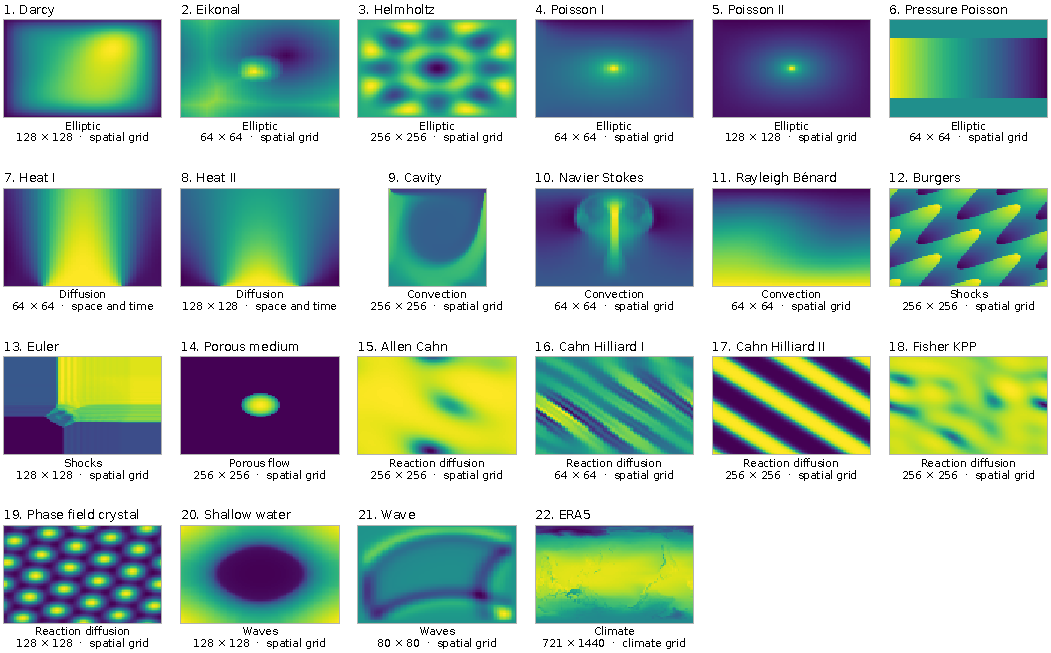
\includegraphics[width=\linewidth]{figures/dataset_gallery.pdf}
\caption{\textbf{The 22 datasets span different field structures.} Panels are
grouped by class and show one fine training field per dataset with its native grid size. Heat fields span space
and time, and the cavity shows vorticity. ERA5 predictions use a
$128\times256$ working grid. Display conventions are described in
Appendix~\ref{app:gallery}. Imported data: Poisson II, Heat II, and Navier Stokes
\citep{niu2024}, and ERA5 \citep{hersbach2020,niu2024}.}
\label{fig:datasets}
\end{figure}

\subsection{Ensemble fitting budgets and evaluation}
For each PDE dataset, we keep the trained models fixed and ask how many
additional fine solutions are needed to choose their mixture. We compare
$K\in\{5,10,20\}$ fitting examples, each consisting of an input and its known
fine field. These examples are separate from surrogate training and evaluation.
Every rule receives the same $K$ examples for selecting an individual model
or fitting mixture weights. We then measure prediction error on
separate evaluation cases shared by all methods. We repeat this comparison
using three partitions of fitting and evaluation cases without retraining
the models. This measures sensitivity to the choice of fitting examples.
Split construction and case counts are given in Appendix~\ref{app:splits}.

We report mean relative $L^2$ error, averaging over cases and then partitions.
To compare proportional changes across datasets, we aggregate error ratios
geometrically. Dataset aggregation gives each dataset equal weight. PDE class
aggregation first averages within each class and then gives the classes equal
weight:
\begin{equation}
 \rho_{a/b}=\exp\!\left[\frac1{|\mathcal C|}\sum_{c\in\mathcal C}
 \frac1{|\mathcal D_c|}\sum_{d\in\mathcal D_c}\log\frac{\bar E_{d,a}}{\bar E_{d,b}}\right].
 \label{eq:aggregate}
\end{equation}
Here $a,b$ denote methods, $\bar E_{d,a}$ is method $a$'s partition averaged error
on dataset $d$, $\mathcal C$ is the set of PDE classes, and $\mathcal D_c$ contains
class $c$'s datasets. Vertical bars count set members. The ratio $\rho_{a/b}$ gives
each class equal weight, with values below one favoring $a$. The two summaries answer
different questions: a dataset in a singleton class has six times the weight
of one elliptic dataset under class aggregation. Wins and losses require more
than a 1\% relative change. This is a descriptive threshold, not a significance
test. Tables express errors as percentages and improvements as relative changes.
